\chapter{แนวคิด ทฤษฎีและงานวิจัยที่เกี่ยวข้อง}
\label{chapter:related-theory}

\section{การตรวจหาข้อความในภาพถ่ายด้วยเทคนิค Stroke Width Transform}

วิธีการการตรวจหาข้อความในภาพถ่าย~\cite{5540041} นี้เป็นวิธีการที่เรานำมาใช้ศึกษาและเป็นต้นแบบในการพัฒนาเพื่อทำงานร่วมกับภาพมังงะ  โดยมีขั้นตอนทั้งหมดแบ่งได้เป็น 3 ขั้นตอน ขั้นแรกคือการใช้ Stroke Width Transform ในการปรับเปลี่ยนข้อมูลให้แสดงลักษณะของความกว้างในแต่ละเส้นภายในภาพ ขั้นที่สอง ค้นหาวัตถุที่คล้ายคลึงกับตัวอักษรในภาพโดยใช้กฎเกณฑ์ที่กำหนดไว้ ขั้นสุดท้าย คือ การจัดกลุ่มตัวอักษรเข้าด้วยกันเป็นบรรทัดของข้อความ

\subsection{Stroke Width Transform}

Stroke Width Transform หรือ SWT เป็นเทคนิคที่ใช้ช่วยในการทำงานของระบบตรวจหาข้อความในภาพถ่าย โดยสกัดลักษณะเด่นของเส้นต่าง ๆ ในภาพ เช่น เส้นของตัวอักษร เป็นต้น~\cite{5540041} ด้วยลักษณะดังกล่าว ทำให้เราสามารถใช้ในการคัดแยกวัตถุที่เป็นตัวอักษรออกจากวัตถุอื่น ๆ ได้โดยพึ่งพาลักษณะเด่นเหล่านั้น

เริ่มแรกเราสร้างภาพ Output ที่มีขนาดเท่ากับภาพที่ต้องการตรวจหาข้อความ โดยแต่ละ Pixel ในภาพถูกกำหนดให้มีค่าอนันต์ ($\infty$) จากนั้นใช้ Canny Edge Detection~\cite{4767851} ตรวจหาตำแหน่งของขอบของวัตถุในภาพ ซึ่งจากตัวอย่างในภาพ หากเรามีภาพ~\ref{Fig:swt:a} จากนั้นใช้การตรวจหาตำแหน่งขอบของวัตถุ เราจะได้ผลลัพธ์ตามภาพ~\ref{Fig:swt:b} เมื่อตรวจหาตำแหน่งขอบเสร็จสิ้นต่อมาจะคำนวนความกว้างของเส้นโดยใช้ขอบที่ได้มา ความกว้างคำนวนได้จากระยะห่างระหว่างขอบของเส้นโดยพิจารณาทุก Pixel $p$ ของขอบที่ได้จาก Canny Edge Detection เพื่อหา Pixel $q$ ที่เข้าคู่กัน อย่างที่แสดงให้เห็นในภาพ~\ref{Fig:swt:b} การหา $q$ จาก $p$ ทำได้โดยใช้ Gradient Direction ของ $p$ ซึ่งคือ $d_p$ โดย $d_p$ จะชี้ไปหา $q$ และหาก $d_p$ และ $d_q$ มีทิศทางตรงกันข้ามโดยประมาณ $d_q = -d_p \pm \pi/6$ ให้กำหนดค่าให้กับแต่ละ Pixel ที่อยู่ภายใต้แนวทางระหว่าง $p$ และ $q$ ให้มีค่าเท่ากับ $\| \overrightarrow{p-q}\|$ เว้นแต่ว่า Pixel ที่จะระบุค่าให้นั้นมีค่าเดิมน้อยกว่าค่าใหม่ที่จะระบุให้ ดังนั้นหากค่าใหม่น้อยกว่าค่าเดิมใน Pixel ก็สามารถทำการระบุค่าใหม่แทนทีค่าเดิมให้กับ Pixel นั้นได้ อย่างที่ปรากฎในภาพ~\ref{Fig:swt:c} เมื่อทำครบทุก Pixel ในภาพ สุดท้ายจะได้เมทริกซ์ Output ขนาดเท่าภาพ Input โดยมีค่าของความกว้างเส้นถูกระบุในพื้นที่ระหว่างขอบของเส้นอย่างเช่นปรากฏในภาพ~\ref{Fig:swt:c}

\begin{figure}[!h]
    \centering
    \subfigure[]{
        \label{Fig:swt:a}
        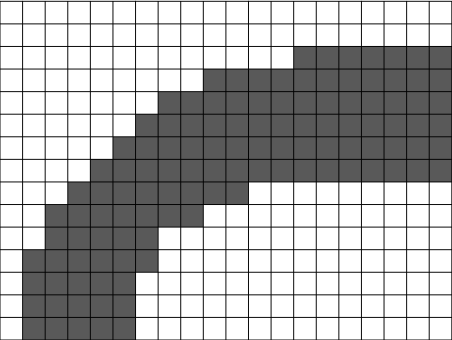
\includegraphics[width=0.4\textwidth]{swt-a.png}  
    }
    \subfigure[]{
        \label{Fig:swt:b}
        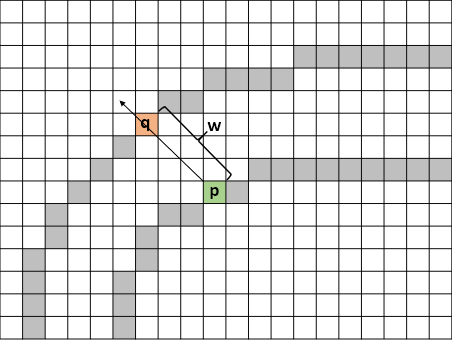
\includegraphics[width=0.4\textwidth]{swt-b.png}  
    }
    \subfigure[]{
        \label{Fig:swt:c}
        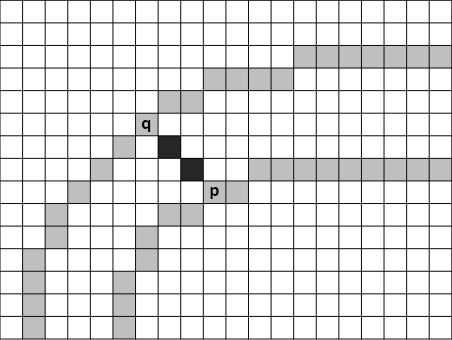
\includegraphics[width=0.4\textwidth]{swt-c.png}  
    }
    \caption{ขั้นตอนการทำงานของ Stroke Width Transform}
    \label{Fig:swt}
\end{figure}

\subsection{ค้นหาวัตถุที่มีลักษณะใกล้เคียงตัวอักษร}

ในขั้นตอนนี้เรานำผลลัพธ์จากขั้นตอนก่อนหน้ามากำจัดวัตถุที่ไม่มีลักษณะคล้ายคลึงอักษร เริ่มจากจับกลุ่มแต่ละ Pixel ในผลลัพธ์ของขั้นตอนก่อนหน้า การจับกลุ่มทำได้โดยเปรียบเทียบแต่ละ Pixel กับ Pixel เพื่อนบ้านรอบข้าง หาก Pixel สองตัวที่เปรียบเทียบกันมีค่าของความกว้างเส้นไม่ต่างกันเกิน 3.0  เท่า ให้ถือว่า Pixel ทั้งสองเป็นส่วนของวัตถุเดียวกันซึ่งจะถูกจัดกลุ่มเข้าด้วยกัน เมื่อการจัดกลุ่ม Pixel เสร็จสิ้น ผลลัพธ์ที่ได้คือภาพวัตถุต่าง ๆ ที่ปรากฏในภาพหรือ Connected Components อย่างไรก็ดีหากวัตถุที่เกิดจากการรวมกลุ่มของ Pixel นั้นใหญ่หรือเล็กเกินไปก็จะถูกคัดออก การคัดวัตถุลักษณะดังกล่าวออกไปทำโดยการใช้กฎสองข้อดังนี้ (\rNum{1}) อัตราส่วนระหว่างเส้นผ่าศูนย์กลางต่อมัธยฐานของความกว้างของเส้นตัวอักษรนั้นต้องน้อยกว่า 10  (\rNum{2}) ความสูงต้องมากกว่า 10 และน้อยกว่า 300 ตามที่แสดงในสมการ~\ref{eq:old-condition}


\begin{equation}
f(d, h, \tilde{s})= 
\begin{cases}
1, &\text{if } \frac{d}{\tilde{s}} < 10 \text{ and } 10 < h < 300\\
0, &otherwise
\end{cases},
\label{eq:old-condition}
\end{equation}

โดย $d$ คือ เส้นผ่าศูนย์กลางของวัตถุ, $h$ คือ ความสูงของวัตถุ, และ $\tilde{s}$ คือ มัธยฐานของของความกว้างเส้นตัวอักษร โดยค่าความกว้างได้มาจากค่าของ Pixel ในพื้นที่ของเส้นที่ถูกระบุไปโดยขั้นตอน SWT

\subsection{จัดกลุ่มตัวอักษร}

วัตถุแต่ละชิ้นที่ทีลักษณะคล้ายคลึงกับอักษรซึ่งผ่านการคัดกรองด้วยกฎจากขั้นตอนก่อนหน้าจะถูกนำมาจับกลุ่มเป็นบรรทัดของข้อความในขั้นตอนนี้โดยใช้การเปรียบเทียบความคล้ายคลึงระหว่างลักษณะอักษรต่าง ดังนี้ ระยะห่างระหว่างวัตถุ, อัตราส่วนความกว้างของเส้นอักษร, และความสูงของอักษร โดยสองวัตถุจะถูกจัดกลุ่มกันต่อเมื่อ (\rNum{1}) อัตราส่วนระหว่างค่ามัธยฐานความกว้างเส้นของวัตถุทั้งสองมีค่าน้อยกว่า 2 เท่า (\rNum{2}) ความสูงของอักษรทั้งสองต่างกันไม่เกิน 2 เท่า (\rNum{3}) ระยะห่างระหว่างสองวัตถุนั้นมีค่าไม่เกิน 3 เท่าของวัตถุที่กว้างที่สุดในคู่อักษรที่ใช้เปรียบเทียบ หลังจากการจัดกลุ่มนี้เราจะได้โซ่ของอักษรที่ถูกจัดกลุ่มเข้าด้วยกัน แต่ละโซ่ประกอบไปด้วยอักษรสองตัวที่ถูกจัดกลุ่ม ต่อมานั้นแต่ละโซ่จะถูกรวมเข้าด้วยกันหากโซ่อักษรมีอักษรในโซ่ของตนร่วมกันโซ่อื่น ๆ และทิศทางของโซ่มีความใกล้เคียงกัน

สุดท้ายขั้นตอนนี้จะจบลงเมื่อไม่มีโซ่อักษรใด ๆ ถูกเชื่อมต่อเพิ่มเติม ในที่สุดเราจะได้กลุ่มหรือโซ่ของอักษรที่เกิดจากการจัดกลุ่มด้วยความคล้ายคลึงของอักษรและทิศทางของข้อความ อีกนัยนึงคือเราได้กลุ่มบรรทัดของแต่ละประโยคออกมาจากภาพถ่ายเรียบร้อยในขั้นตอนนี้

\section{Histogram of Oriented Gradients}

Histogram of Oriented Gradients (HOG) เป็นการสกัด Feature ของภาพโดยอาศัยรูปแบบ Histogram ของทิศทางเฉดสีในภาพ หรือ Gradient direction เพื่อพิจารณาลักษณะของวัตถุต่าง ๆ อย่างที่แสดงในภาพ~\ref{Fig:hog} โดยภาพ~\ref{Fig:hog:letter} คือ ตัวอย่างอักษรภาษาญี่ปุ่น และภาพ~\ref{Fig:hog:hog} คือภาพแสดงทิศทางของเฉดสีของภาพอักษรโดยใช้เส้นขนาดเล็กแสดงทิศทางของเฉดสี ด้วยความสามารถนี้ จึงมีการนำ HOG มาใช้สำหรับสกัดลักษณะเด่นเพื่อใช้ในงานจำพวกการตรวจจับวัตถุอย่างหลากหลาย ทั้ง การตรวจจับท่าทางของมือ~\cite{Freeman}, การตรวจจับรถบนท้องถนน~\cite{8314922}, การตรวจจับมนุษย์ในภาพ~\cite{1467360} และไม่เพียงแค่สามารถใช้กับงานตรวจจับวัตถุ แต่ยังสามารถใช้กับงานด้านตรวจหาข้อความในภาพได้เช่นกัน~\cite{DBLP:journals/corr/WangWZLZ15, 6628751, 8280697}

\begin{figure}[!h]
    \centering
    \subfigure[]{
        \label{Fig:hog:letter}
        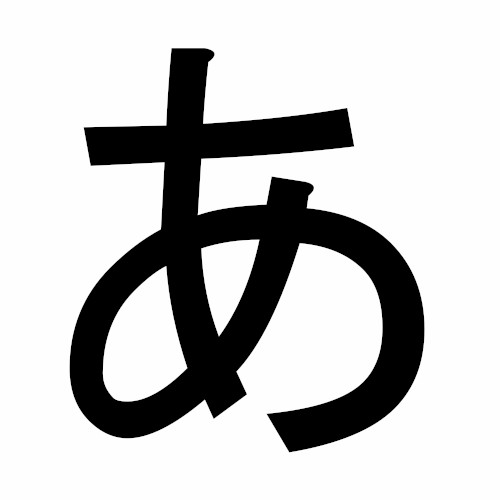
\includegraphics[width=0.45\textwidth]{letter.jpg}  
    }
    \subfigure[]{
        \label{Fig:hog:hog}
        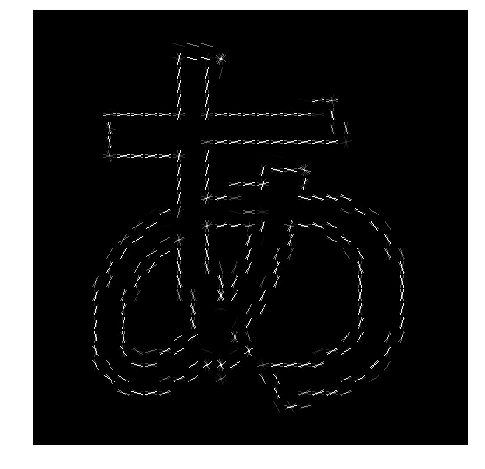
\includegraphics[width=0.45\textwidth]{hog.png}  
    }
    \caption{ตัวอย่างข้อมูลนำเข้าและการจำลองภาพทิศทางของ Histogram of Oriented Gradients}
    \label{Fig:hog}
\end{figure}

การสกัดลักษณะเด่นของ HOG นั้นทำได้โดยเริ่มจากแบ่งภาพเป็นส่วนเล็ก เรียกว่า Cell หรือช่องสีแดงตามที่แสดงในภาพ~\ref{Fig:cell-and-block} จากนั้นสร้าง Histogram สำหรับ Cell นั้น ๆ ด้วยค่า Gradient Direction และ Magnitude โดย Histogram นี้จะเป็นตัวแทนของลักษณะขอบและรูปร่างที่อยู่ภายใน Cell นั้น ๆ จากนั้นจะทำการ Normalization กับ Histogram ของแต่ละ Cell ด้วยกลุ่มของ Cell หรือที่เรียกว่า Block อย่างที่เห็นเป็นช่องสีน้ำเงินในภาพ~\ref{Fig:cell-and-block} สุดท้ายเราจะได้ Histogram ของ Gradient Direction จากทุก ๆ Cell ของภาพซึ่งเป็นตัวแทนของรูปร่างวัตถุแต่ละส่วน ด้วย Histogram ที่ได้มาจะถูกนำไปเข้ากระบวนการ Vectorization เพื่อให้สามารถใช้ในงานอื่น ๆ ได้ต่อไป

\begin{figure}[!h]
    \centering
    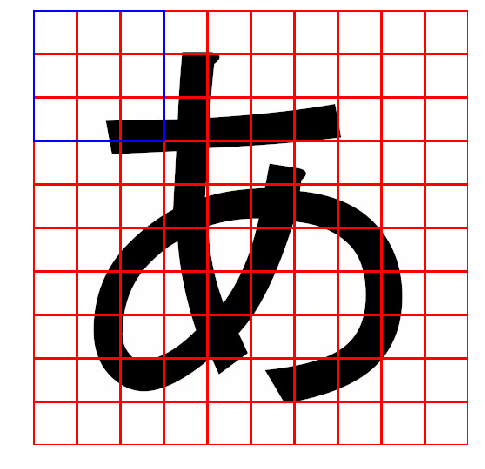
\includegraphics[width=0.45\textwidth]{block.png}  
    \caption{Cell และ Block ในการทำงานของ Histogram of Oriented Gradients}
    \label{Fig:cell-and-block}
\end{figure}

อย่างไรก็ดีการที่จะได้ HOG ของวัตถุที่เราต้องการตรวจสอบจำเป็นต้องใช้ภาพของวัตถุนั้น ๆ ในการคำนวณ แต่ในสถานการณ์จริงภาพของวัตถุอาจอยู่ในภาพถ่ายขนาดใหญ่ที่ประกอบไปด้วยหลายวัตถุ เราจึงต้องตัดภาพของวัตถุเป็นส่วนย่อยเพื่อใช้คำนวณกับ HOG เราเรียกภาพส่วนย่อยที่ถูกตัดออกมานั้นว่า Patch ดังนั้นเราจำเป็นต้องใช้ Patch ที่มีขนาดใกล้เคียงกับวัตถุนั้น ๆ เป็นเหตุให้หากภาพมีขนาดใหญ่แต่วัตถุที่ต้องการตรวจพบมีขนาดเล็ก จำนวน Patch ก็จะมากขึ้น

ในกรณีของมังงะ ตัวอักษรมักมีขนาดเล็ก (20px – 40px โดยส่วนใหญ่อ้างอิงจาก Dataset ของเรา) เมื่อเทียบกับขนาดภาพมังงะ (1170px อ้างอิงจาก dataset ของเรา) ซึ่งมีขนาดใหญ่กว่าหลายเท่า ดังนั้นจำนวนของ Patch ที่ต้องสร้างและคำนวนด้วย HOG จึงมีมหาศาลและสร้างภาระแก่การคำนวน ลักษณะเด่นด้วย SVM อย่างมาก ซึ่งปัญหาส่วนนี้ส่งผลกระทบต่อความเร็วในการทำงานของเรา เราจึงใช้ SWT สำหรับกำหนดพื้นที่ที่คาดว่าเป็นอักษรเพื่อใช้สร้าง Patch แทนการสร้าง Patch จากทุกส่วนของภาพด้วยการใช้ Sliced Window

\section{Support Vector Machine}

Support Vector Machine (SVM)~\cite{Suykens1999} เป็นเทคนิค Pattern Recognition แบบ Supervised Learning ซึ่งถูกใช้ทั้งในงานเพื่อ Classification และ Regression ซึ่งภายในงานนี้ได้ใช้งานเพื่อ Classification โดยทำงานด้วยการสร้าง Hyper-plane ที่เหมาะสมที่สุด (Optimal) เพื่อจำแนกแยกข้อมูลสองกลุ่มอย่างที่แสดงในภาพ~\ref{Fig:svm}

\begin{figure}[!h]
    \centering
    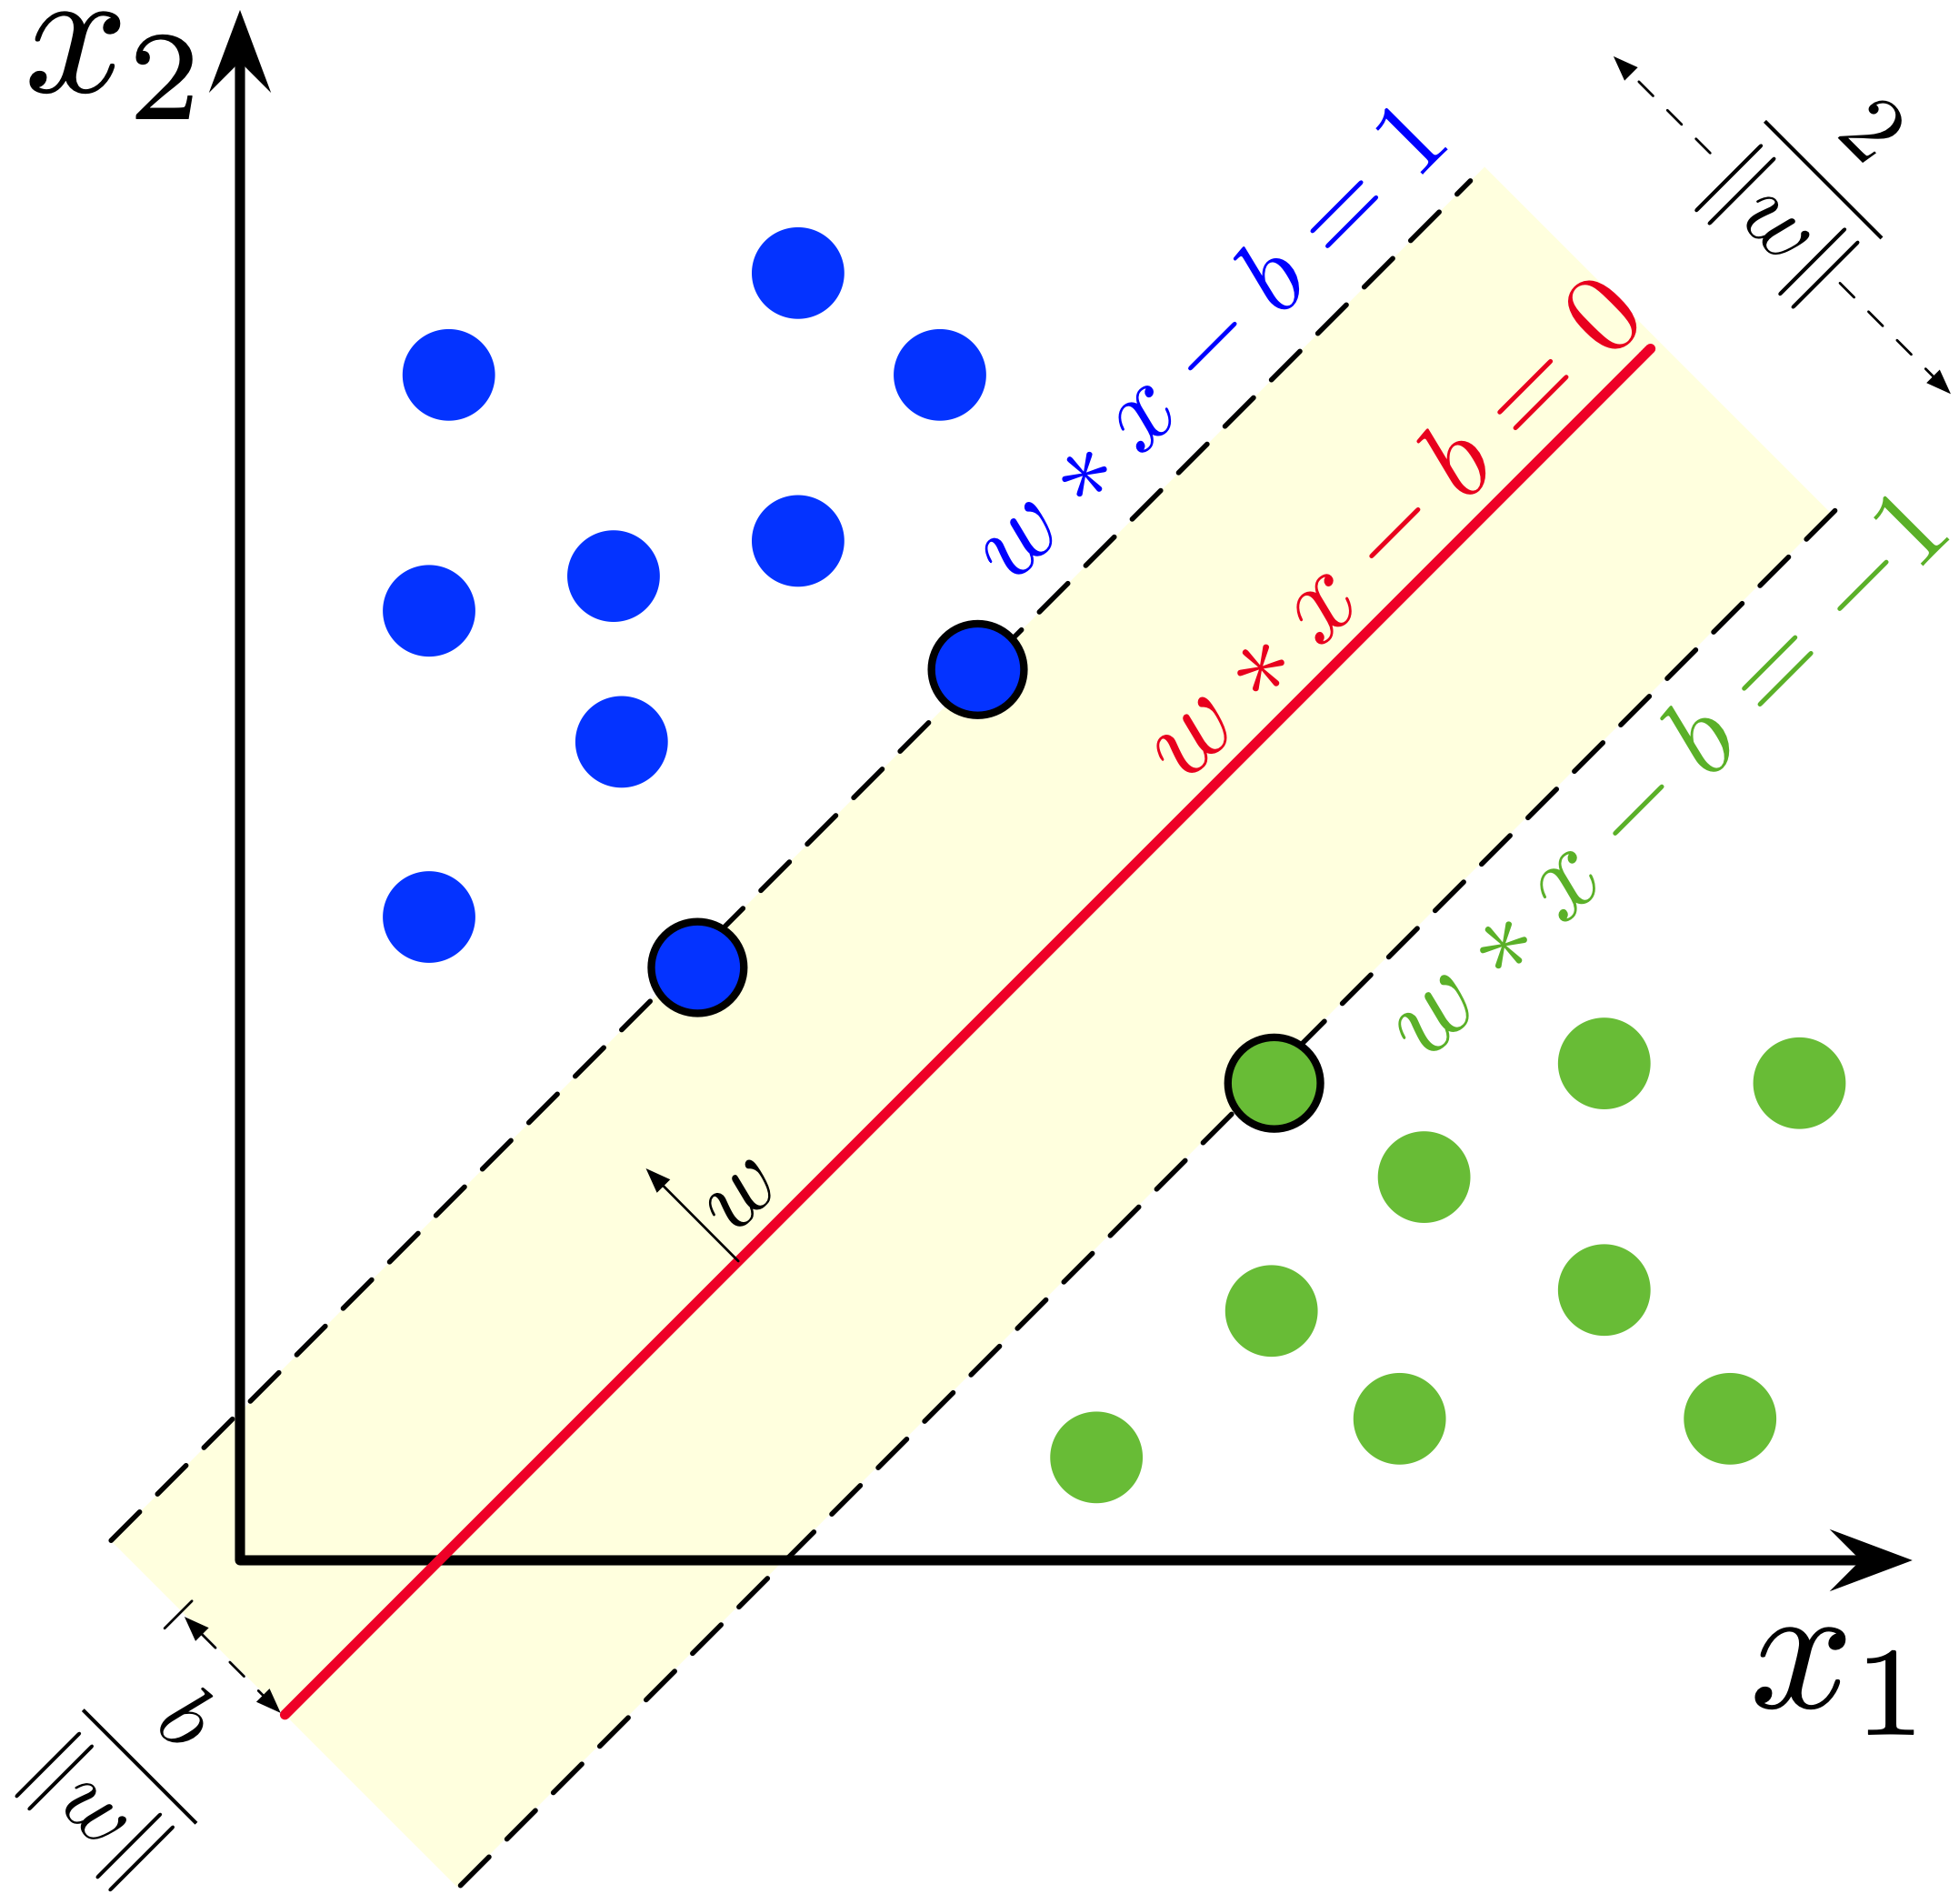
\includegraphics[width=0.5\columnwidth]{svm.png}
    \caption{การแบ่งแยกกลุ่มข้อมูลด้วย Hyper-plane ของ SVM}
    \label{Fig:svm}
\end{figure}

เพื่อที่จะแยกข้อมูลทั้งสองกลุ่มด้วย Optimal Hyper-plane นั้น $w \times x - b = 0$ จะทำหน้าที่แบ่งข้อมูลสองกลุ่มออกจากกันโดยมี Support Vector ทำหน้าที่เป็นกันชนระหว่างข้อมูลที่ใกล้กันที่สุดระหว่างกลุ่มข้อมูลทั้งสอง ซึ่ง SVM นั้นจะสร้างพื้นที่การตัดสินใจขึ้นมา หรือก็คือพื้นระหว่าง $w \times x - b = 1$ และ $w \times x - b = -1$ โดยจะปรับให้ระยะห่างหรือความกว้างระหว่างทั้งสองนั้นมีค่าสูงสุด โดยระยะห่างนั้นมีค่าเท่ากับ $\frac{2}{\|\vec {w}\|}$ อย่างไรก็ดีหลาย ๆ ครั้งข้อมูลไม่สามารถแบ่งแยกได้ด้วยเส้นตรง และจำเป็นต้องใช้การแบ่งข้อมูลแบบ Non-linear ซึ่งสำหรับ SVM แล้วนั้นสามารถใช้ Kernel เข้ามาช่วยในการเปลี่ยนมิติของข้อมูลเพื่อให้สามารถแบ่งแยกข้อมูลทั้งสองกลุ่มได้ด้วย Linear Hyper-plan ตามที่แสดงในภาพ~\ref{Fig:kernel}

\begin{figure}[!h]
    \centering
    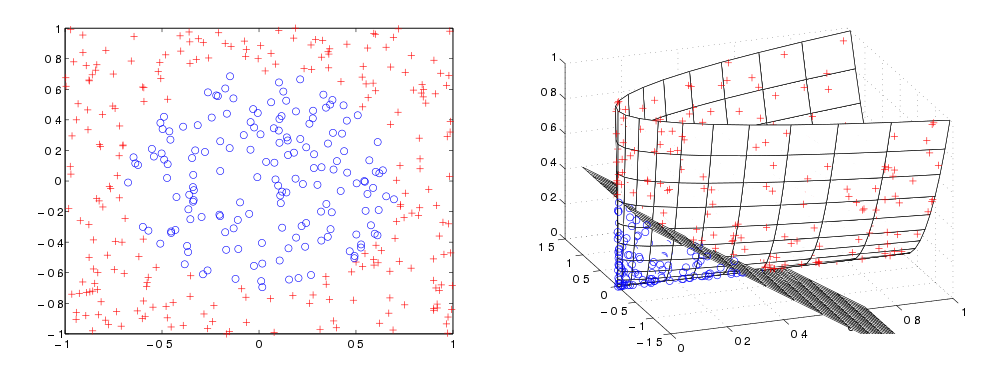
\includegraphics[width=0.95\columnwidth]{kernel.png}
    \caption{คุณสมบัติการเปลี่ยนมิติของข้อมูลด้วย Kernel}
    \label{Fig:kernel}
\end{figure}

